\graphicspath{{content/chapters/7_evaluation/figures/}}
\chapter{Evaluation}
\label{chp:evaluation}

This chapter presents a comprehensive evaluation of the implemented speech enhancement system, assessing both classical and deep learning approaches across several dimensions. The evaluation is divided into three key parts. First, the impact of dataset handling strategies is examined, comparing how the different dataset methods affect training efficiency and performance. Second, the effectiveness of Out-of-Memory (OOM) mitigation techniques is validated to ensure that memory-saving strategies do not degrade model quality. Finally, the core focus of this chapter is a comparative analysis of model architectures, benchmarking five machine learning models against three classical denoising methods. Each section includes detailed quantitative assessments using respective metrics. Results are presented using clear, tabulated formats for ease of interpretation and cross-comparison.

\section{Dataset Performance}
\label{sec:dataset_performance}

This section examines the performance of the three dataset handling strategies: Static Bucketing, Dynamic Bucketing, and Padding-Truncation Output-Truncation (PTO). The goal is to assess how these strategies affect the overall efficiency of the training process, particularly in terms of dataset loading times, runtime overhead during training, and their influence on model performance. Each strategy was tested using the same model architecture, the Contextual Encoder-Decoder (CED), under two conditions:

\begin{itemize}
    \item \textbf{Cold Run (Uncached):} In this scenario, all dataset operations are executed from scratch. Static and Dynamic Bucketing compute bucket assignments (with Dynamic Bucketing also requiring K-Means clustering), while PTO calculates and stores the original waveform lengths. This setup simulates a first-time deployment or training on a fresh system.
    
    \item \textbf{Warm Run (Cached):} This run utilizes cached data generated during the cold run, significantly reducing load and preprocessing time. For Static and Dynamic Bucketing, bucket mappings and K-Means centers are reloaded. For PTO, the previously computed original sequence lengths are retrieved.
\end{itemize}

The configuration used for all CED runs is shown in Figure~\ref{fig:dataset_config}, with the only varying parameter being the \texttt{PAD\_METHOD}.

\begin{figure}[H]
    \centering
    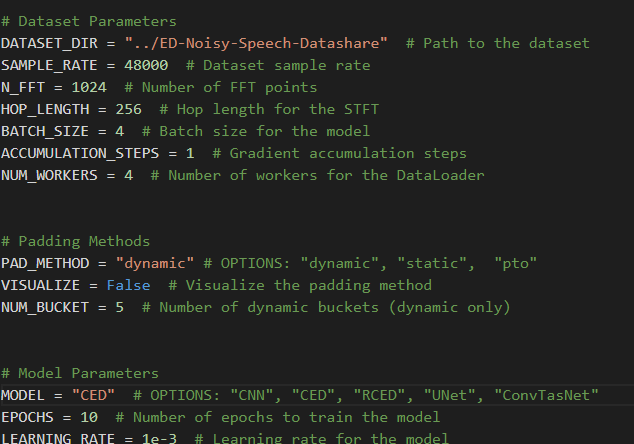
\includegraphics[width=0.8\textwidth]{dataset_config.png}
    \caption{\label{fig:dataset_config} Configuration of the CED model used for dataset performance evaluation.}
\end{figure}

Both uncached and cached runs were executed, and the relevant timing metrics were collected from the output logs, as shown in Table~\ref{tab:dataset_loading_times}.

\vspace{1em}
\begin{table}[H]
\centering
\caption{Dataset Training Overheads}
\label{tab:dataset_loading_times}
\begin{tabular}{|l|c|c|c|}
\hline
\textbf{Dataset} & \textbf{Uncached} & \textbf{Cached} & \textbf{Truncation Overhead} \\
\hline
Static Bucketing  & 298.05 s  & 0.81 s   & N/A    \\
Dynamic Bucketing & 602.56 s& 0.58 s  & N/A    \\
PTO               & 311.21 s & 0.58 s  & 58.56 s  \\
\hline
\end{tabular}
\end{table}

The results in Table~\ref{tab:dataset_loading_times} offer a clear overview of the dataset loading times and runtime overheads associated with each method. Static Bucketing yields the fastest initial loading time, as it involves only dataset loading and bucket assignment. Dynamic Bucketing incurs further overhead due to the computational cost of K-Means clustering. PTO, while slightly slower than Static Bucketing, remains efficient given that it must iterate through the dataset to compute the original waveform lengths.

The re-run loading times for all three methods are significantly reduced due to the use of cached data. All methods show comparable re-run times, with Static Bucketing being marginally slower.

A key distinction lies in the \textit{epoch truncation overhead}. Only the PTO method incurs this overhead due to its need to truncate outputs during training and evaluation to match the original input lengths. This step is unnecessary for the other two methods. While this added runtime is relatively minor compared to the total training duration (typically on the order of hours), this overhead can scale significantly with larger datasets or more training epochs.

To evaluate the impact of dataset handling strategies on model learning, all models were compared using their best training checkpoint. Since the difference between cached and uncached runs was negligible in terms of performance, only the cached results are reported in Table~\ref{tab:dataset_performance}.

\vspace{1em}
\begin{table}[H]
\centering
\caption{Dataset Handling Strategies Training Metrics}
\label{tab:dataset_performance}
\begin{tabular}{|l|c|c|c|}
\hline
\textbf{Dataset} & \textbf{Train Loss} & \textbf{Val Loss} & \textbf{Val SNR} \\
\hline
Static Bucketing  & 0.8367  & 0.8410  & 1.09 dB \\
Dynamic Bucketing & 0.8262  & 0.8298  & 1.10 dB \\  
PTO               & 0.6288  & 0.6633  & 1.10 dB \\
\hline
\end{tabular}
\end{table}

The results in Table~\ref{tab:dataset_performance} indicate that the model achieves comparable performance across all dataset handling methods. The consistent validation SNR values suggest correct implementation across all strategies and indicate that the model learned equivalent representations irrespective of the input formatting.

Interestingly, the PTO method shows a slightly lower training and validation loss. This discrepancy is not reflected in the SNR metric and may be attributed to differences in how output sequences are truncated during training. Causing the average loss to be lower than the other two methods. However, this does not translate into improved denoising performance, as indicated by the similar SNR values.

While all three methods enable effective training, Dynamic Bucketing offers the most balanced trade-off. It adapts well to the dataset’s variable-length distribution, minimizes unnecessary padding, and avoids the runtime overhead introduced by PTO. Therefore, Dynamic Bucketing is selected as the preferred method for the remainder of this project.

\section{OOM Validation}
\label{sec:oom_validation}

While Section~\ref{sec:oom_handling} outlined several techniques to mitigate Out-of-Memory (OOM) errors during training. It is important to demonstrate that these strategies do not compromise model learning. The goal of this section is to validate that memory-saving methods do not lead to information loss or degraded performance. To assess this, three training configurations were evaluated using the same RCED model architecture and the Dynamic Bucketing dataset strategy:

\begin{enumerate}
    \item \textbf{Clean Training (Baseline):} A standard training loop without any OOM-handling logic, using a batch size of 4. This configuration serves as the control, with no memory management mechanisms.
    
    \item \textbf{OOM Handling (Batch 4, Accum 1):} OOM-handling techniques were enabled while maintaining a batch size of 4. These included fixed-point precision (FP16) and garbage collection (GC), allowing for a more memory-efficient training process.
    
    \item \textbf{OOM + Accumulation (Batch 2, Accum 2):} The batch size was reduced to 2, with gradient accumulation set to 2, simulating an effective batch size of 4. All OOM-handling techniques remained enabled. This configuration is designed to reduce memory usage while preserving gradient stability.
\end{enumerate}

Each configuration was trained for the same number of epochs, using identical learning rates, optimizers, and data augmentation (if any). Table~\ref{tab:oom_training} summarizes the training and validation performance.

\vspace{1em}
\begin{table}[H]
\centering
\caption{OOM Configurations Training Metrics}
\label{tab:oom_training}
\begin{tabular}{|l|c|c|c|c|}
\hline
\textbf{Train Config} & \textbf{Train Loss} & \textbf{Val Loss} & \textbf{Val SNR} & \textbf{Training Time} \\
\hline
Baseline               & 0.7985 & 0.8048 & 1.12 dB & 4.24 h \\
OOM Handling           & 0.8026 & 0.8077 & 1.11 dB & 2.58 h \\
OOM + Accumulation     & 0.8007 & 0.8077 & 1.11 dB & 3.02 h \\
\hline
\end{tabular}
\end{table}

As shown in Table~\ref{tab:oom_training}, OOM-handling techniques do not significantly affect model performance. Although the training and validation losses are slightly higher than the baseline, the differences are minimal and are outweighed by the substantial reduction in training time. This speedup likely results from improved memory efficiency via FP16 computation, garbage collection, and reduced GPU memory overhead.

Each model was also evaluated in the full denoising pipeline. Table~\ref{tab:oom_metrics} presents the performance metrics across key evaluation criteria.

\vspace{1em}
\begin{table}[H]
\centering
\caption{OOM Configurations Denoising Metrics}
\label{tab:oom_metrics}
\begin{tabular}{|l|c|c|c|c|c|}
\hline
\textbf{Train Config} & \textbf{↑SNR} & \textbf{↓MSE} & \textbf{↑PESQ} & \textbf{↑STOI} & \textbf{↓LSD} \\
\hline
Baseline               & 0.9751 & 0.002083 & 1.3867 & 0.8205 & 0.7857 \\
OOM Handling           & 0.9648 & 0.002088 & 1.2244 & 0.8037 & 1.0361 \\
OOM + Accumulation     & 0.9714 & 0.002085 & 1.2611 & 0.8044 & 0.9004 \\
\hline
\end{tabular}
\end{table}

Once again, the results in Table~\ref{tab:oom_metrics} confirm that OOM-handling techniques do not degrade model output quality in any meaningful way. The baseline configuration achieves slightly better metrics, which may be attributed to the longer training duration and use of full-precision computation. However, the differences are negligible, and the gains in training efficiency justify the use of OOM-handling strategies in practice.

\section{Model Performance}
\label{sec:model_performance}

This section presents the most critical part of the evaluation and the central focus of the project: a comparative assessment of classical methods and five machine learning models for speech enhancement. Unlike earlier evaluations, which focused on dataset handling strategies and OOM mitigation techniques using fixed models to conduct the justification. The main scope of this project is to justify the use of machine learning models for speech enhancement, and to evaluate their performance against classical methods.


The evaluation retains the previously established dynamic bucketing and OOM handling strategies but now focuses on how model design impacts training efficiency and denoising performance. The section begins with an analysis of classical denoising methods to establish a meaningful baseline for comparison.

\subsection{Classical Methods}
\label{sec:classical_methods}

The classical methods evaluated include Spectral Subtraction (SS), Wiener Filtering (WF), and the Minimum Mean Square Error - Log Spectral Amplitude estimator (MMSE-LSA), all implemented in a single-channel setting. SS and WF 
foundational methods in literature, whilst MMSE-LSA represents a more developed and perceptually motivated approach. Since these methods do not require training, the classical evaluation bypasses training and instead focuses solely on denoising performance using the same pipeline and evaluation metrics as the learning-based models.


\vspace{1em}
\begin{table}[H]
\centering
\caption{Classical Denoised Metrics}
\label{tab:classical_metrics}
\begin{tabular}{|l|c|c|c|c|c|c|}
\hline
\textbf{Method} & \textbf{↑SNR} & \textbf{↓MSE} & \textbf{↑PESQ} & \textbf{↑STOI} & \textbf{↓LSD} & \textbf{Denoise Time} \\
\hline
SS          & 1.5406 & 0.002210 & 1.4574 & 0.8538 & 0.7747 & 01.17 m \\
WF          & -3.3796 & 0.006702 & 1.8721 & 0.8968 & 0.9278 & 01.33 m \\
MMSE-LSA    & -2.3929 & 0.005440 & 2.0671 & 0.8974 & 0.8274 & 01.51 m \\
\hline
\end{tabular}
\end{table}


The results in Table~\ref{tab:classical_metrics} highlight key trade-offs between signal fidelity and perceptual quality. SS achieved the best SNR and MSE, suggesting strong numerical suppression of noise. However, it underperformed in perceptual metrics, likely due to spectral distortion and residual artifacts introduced by aggressive subtraction.

In contrast, WF and MMSE-LSA lacked the same level of numerical suppression. The indicated negative SNR tells us that numerically the denoised signal is noisier than the original clean signal. This may stem from the fact that both methods are designed to enhance perceptual quality rather than numerical accuracy. Clearly shown by the PESQ and STOI scores, which are significantly higher than those of SS. These results support MMSE-LSA's design as the most effective classical method overall, attributed to its perceptually motivated approach. Notably, all classical methods completed denoising in under two minutes, indicating no significant differences in computational cost.

\subsection{Training The ML Models}
\label{sec:training_ml_models}

With the classical methods evaluated, the focus now shifts to the machine learning models. These models were trained using the same dataset handling strategies and OOM mitigation techniques previously established. Each model followed a consistent training configuration: a batch size of 2, accumulation steps of 4, 25 training epochs, and a learning rate of $1 \times e^{-3}$. The table below summarizes the training performance for each model.

\vspace{1em}
\begin{table}[H]
\centering
\caption{Machine Learning Models Training Metrics}
\label{tab:ml_training}
\begin{tabular}{|l|c|c|c|c|}
\hline
\textbf{Model} & \textbf{Train Loss} & \textbf{Val Loss} & \textbf{Val SNR} & \textbf{Training Time} \\
\hline
CNN         & 0.8813 & 0.8883 & 1.06 dB & 3.22 h \\
CED         & 0.8302 & 0.8334 & 1.10 dB & 5.27 h \\
RCED        & 0.8001 & 0.8071 & 1.11 dB & 7.32 h \\
UNet        & 0.7941 & 0.8003 & 1.12 dB & 14.32 h \\
ConvTasNet  & 0.0764 & 0.0760 & 4.76 dB & 13.09 h \\
\hline
\end{tabular}
\end{table}

The results in Table~\ref{tab:ml_training} reveal a steady trend. As the model complexity increases, training and validation losses generally decrease while validation SNR improves. This gradual improvement is particularly evident when moving from CNN to UNet. The CNN model was introduced as a simple baseline to validate the project’s training and evaluation pipeline. Despite its minimal architecture, it delivered solid performance and served as a reference point for more advanced models. The training plot in Figure~\ref{fig:cnn_training_plot} provides a quick visual overview of the model's learning progression. Although a small gap between training and validation loss is observed, which might suggest mild overfitting. The magnitude of this gap (0.007) is negligible, and the model retains good generalization performance, making it a reliable benchmark. A similar trend is observed across the remaining models, with no significant signs of overfitting.

\begin{figure}[H]
    \centering
    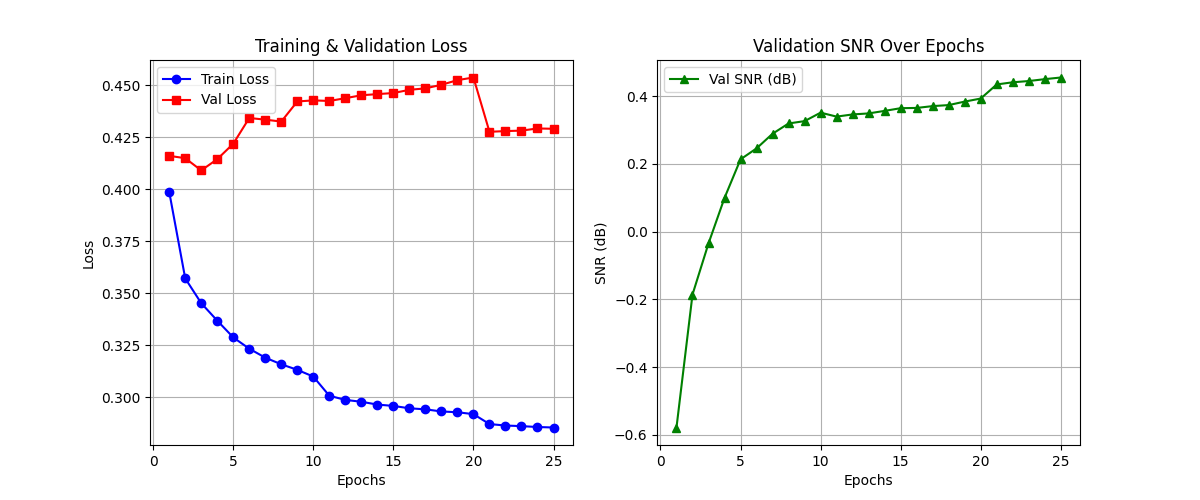
\includegraphics[width=0.8\textwidth]{CNN_plot.png}
    \caption{\label{fig:cnn_training_plot} CNN training plot.}
\end{figure}

The CED and RCED models, adapted from \cite{park2017acoustic}, are encoder-decoder architectures designed specifically for speech enhancement in the spectrogram domain. CED follows a standard encoder-decoder structure, while RCED incorporates residual connections to improve information flow and mitigate vanishing gradient issues.

\begin{figure}[H]
    \centering
    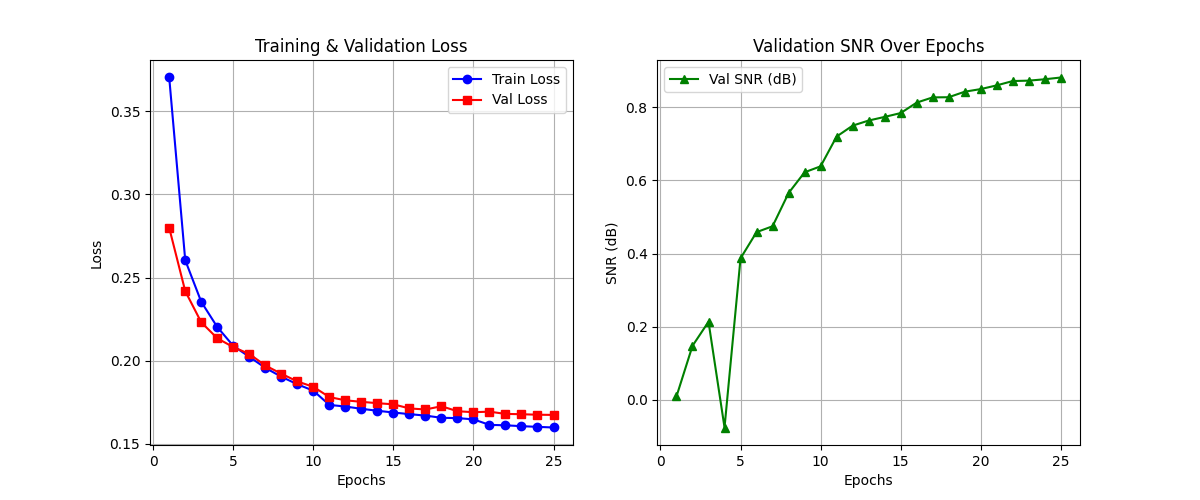
\includegraphics[width=0.8\textwidth]{CED_plot.png}
    \caption{\label{fig:ced_training_plot} CED training plot.}
\end{figure}

\begin{figure}[H]
    \centering
    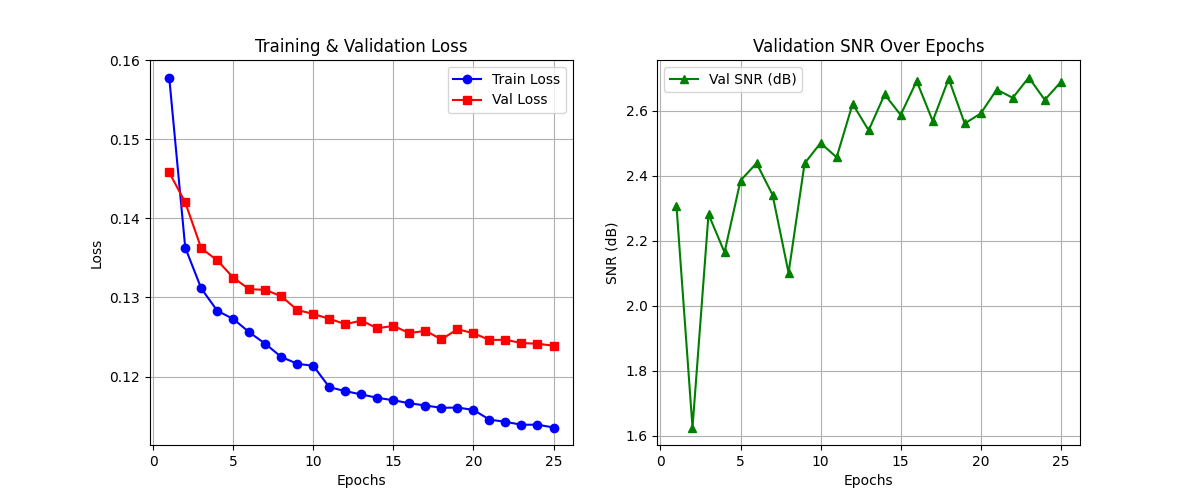
\includegraphics[width=0.8\textwidth]{RCED_plot.png}
    \caption{\label{fig:rced_training_plot} RCED training plot.}
\end{figure}

Confirming the paper’s statement, RCED outperformed CED slightly across training metrics, not with standing the increased training time due to its added complexity. The UNet model, a widely used deep learning architecture, required the longest training time, with once again marginal performance gains.

\begin{figure}[H]
    \centering
    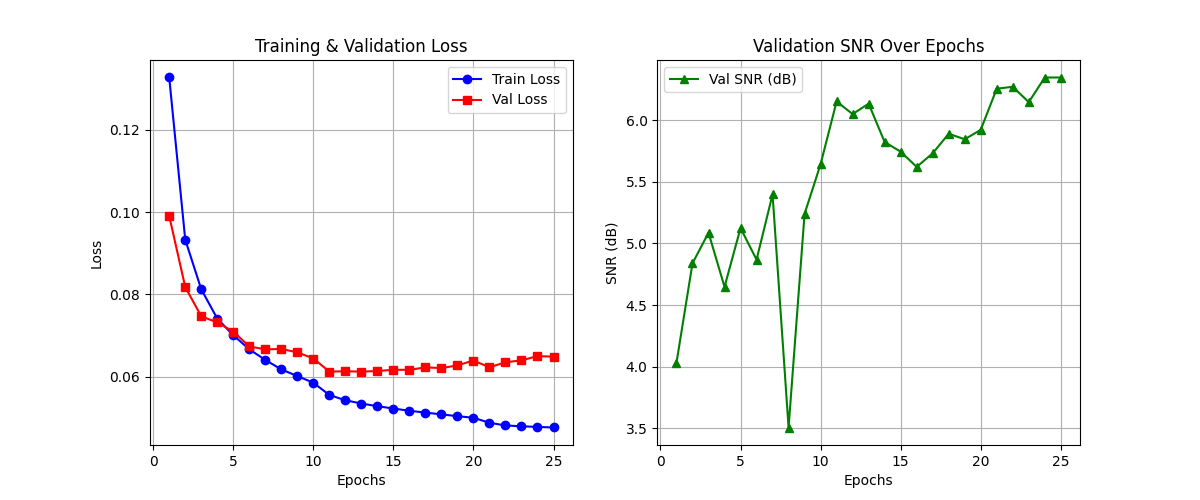
\includegraphics[width=0.8\textwidth]{UNet_plot.png}
    \caption{\label{fig:unet_training_plot} UNet training plot.}
\end{figure}

The most notable result came from ConvTasNet, which showed a significant leap in validation SNR from 1.12 dB (in UNet) to 4.76 dB. This dramatic improvement highlights the architecture’s effectiveness in capturing temporal and spectral signal structure. While loss values alone may not fully reflect denoising capability, ConvTasNet’s results suggest it is learning meaningful representations that translate to superior performance.

\begin{figure}[H]
    \centering
    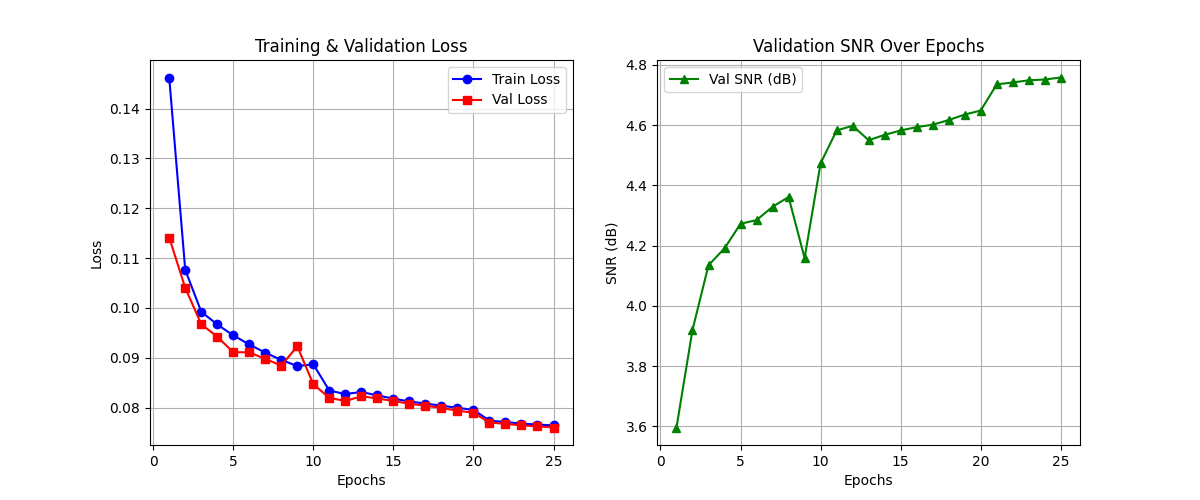
\includegraphics[width=0.8\textwidth]{ConvTasNet_plot.png}
    \caption{\label{fig:convtasnet_training_plot} ConvTasNet training plot.}
\end{figure}

\subsection{Denoising The ML Models}
\label{sec:denoising_ml_models}

Following the training phase, each machine learning model was evaluated using the same denoising pipeline and metrics used for the classical methods. The table below summarizes the performance of all five models across objective and perceptual metrics, as well as their denoising runtime.

\vspace{1em}
\begin{table}[H]
\centering
\caption{Machine Learning Denoising Metrics}
\label{tab:ml_denoise}
\begin{tabular}{|l|c|c|c|c|c|c|}
\hline
\textbf{Model} & \textbf{↑SNR} & \textbf{↓MSE} & \textbf{↑PESQ} & \textbf{↑STOI} & \textbf{↓LSD} & \textbf{Denoise Time} \\
\hline
CNN         & 0.4715  & 0.002340 & 1.1906 & 0.7351 & 0.9639 & 01.28 m \\
CED         & 0.8615  & 0.002138 & 1.1626 & 0.7847 & 0.9210 & 01.24 m \\
RCED        & 0.9655  & 0.002088 & 1.2825 & 0.8115 & 0.9031 & 01.29 m \\
UNet        & 0.9844  & 0.002079 & 1.3273 & 0.7983 & 0.9206 & 01.38 m \\
ConvTasNet  & 17.9050 & 0.000063 & 2.3001 & 0.9001 & 0.6881 & 01.44 m \\
\hline
\end{tabular}
\end{table}

The results in Table~\ref{tab:ml_denoise} show the performance progression across models, reflecting implementation improvements made during the project. The baseline CNN model delivers reasonable perceptual quality out of the box but underperforms in terms of SNR. While its MSE remains close to those of the CED and RCED models, its SNR is nearly halved. Since SNR and MSE are mathematically related in that both measure the difference between the clean and denoised signals. This discrepancy suggests that the CNN is likely retaining higher-energy residual noise. Although the total error magnitude (MSE) may be similar, the CNN's denoised output likely introduces noise that disproportionately affects the signal's energy ratio, thus reducing the SNR. This highlights the importance of evaluating both energy based and perceptual metrics in tandem, as the CNN still maintains moderate PESQ and STOI scores despite its weaker SNR performance.

The CED and RCED models, both adapted from \cite{park2017acoustic}, were introduced to address limitations seen in the CNN baseline. By adopting an encoder-decoder architecture, CED is better suited to the structured nature of spectrograms and is able to capture broader contextual information. This results in a clear improvement in SNR (\textbf{0.86 dB}) compared to CNN (\textbf{0.47 dB}), effectively resolving the earlier energy imbalance issue. RCED builds on this by adding residual connections between layers, which help preserve information flow and stabilize gradient propagation during training. This modification leads to further gains across all metrics, with RCED achieving higher PESQ (\textbf{1.28}) and STOI (\textbf{0.81}) than both CNN and CED, while also slightly improving MSE and SNR.

These results are consistent with the original findings in the Park \textit{et al.} paper, where residual connections were shown to improve performance in speech enhancement tasks. Despite their improvements, both CED and RCED architectures have structural limitations. The use of a single bottleneck without feature merging across scales can lead to a loss of fine-grained spectral detail during encoding and decoding. While RCED mitigates this to some extent through residual connections, it still lacks the explicit skip connections found in UNet, which allow for high-resolution features to be reintroduced at each decoding stage. 

The UNet model extends the encoder-decoder structure by introducing those skip connections. Helping recover fine-grained spectral details lost during downsampling and improves the model’s ability to capture both local and global context. In terms of performance, UNet shows continued gains over its predecessors. It achieves the lowest MSE among the encoder-decoder models, along with a slight improvement in SNR (\textbf{0.98 dB}) and the highest PESQ score (\textbf{1.33}) before ConvTasNet. These results validate the effectiveness of UNet’s multi-scale feature integration. However, the improvement over RCED is modest, indicating diminishing returns as architectural complexity increases. Additionally, UNet requires the longest training time of all models evaluated. Suggesting that while effective, its efficiency-performance tradeoff may not be ideal for all deployment scenarios.

While each machine learning model introduced architectural improvements and showed incremental gains across metrics, the overall progression remained modest. From CNN to UNet, improvements in PESQ, STOI, and SNR were consistently observed, but these came at the cost of increased model complexity and training time. Notably, none of these models achieved a clear breakthrough in performance over the best classical method MMSE-LSA, particularly in perceptual quality. This raises an important consideration: without a significant performance leap, the added training burden and architectural complexity of these models may not be fully justified for real-world deployment.

To address this gap, a model was needed that could scale the benefits of deep learning effectively. One that could translate increased complexity into substantial performance gains. ConvTasNet fulfilled this requirement. Although it incurred the second-highest training time among all models, it delivered a dramatic improvement across all evaluation metrics. Most notably, it achieved an SNR of \textbf{17.91 dB}, far exceeding the incremental gains observed in previous models, and outperformed all others in PESQ (\textbf{2.30}) and STOI (\textbf{0.90}).

Although originally introduced as a time-domain separation network in \cite{Luo2018ConvTasNetSI}, ConvTasNet was adapted in this project to operate directly on spectrograms, using 2D convolutions over the real and imaginary components. This adjustment allows the model to remain compatible with the spectrogram-based pipeline used throughout the project, while still leveraging ConvTasNet’s core strength. Its stacked temporal convolutional blocks with dilation and residual connections. These features enable the model to capture long-range dependencies across time and frequency axes effectively. Given its exceptional results and practical inference time, ConvTasNet was ultimately selected for deployment in this project. 